% !TEX encoding = UTF-8 Unicode
\documentclass[10pt]{standalone}\usepackage{tikz}
\usepackage{fontspec}
\setmainfont{Arial}
\setsansfont{Arial}\begin{document}

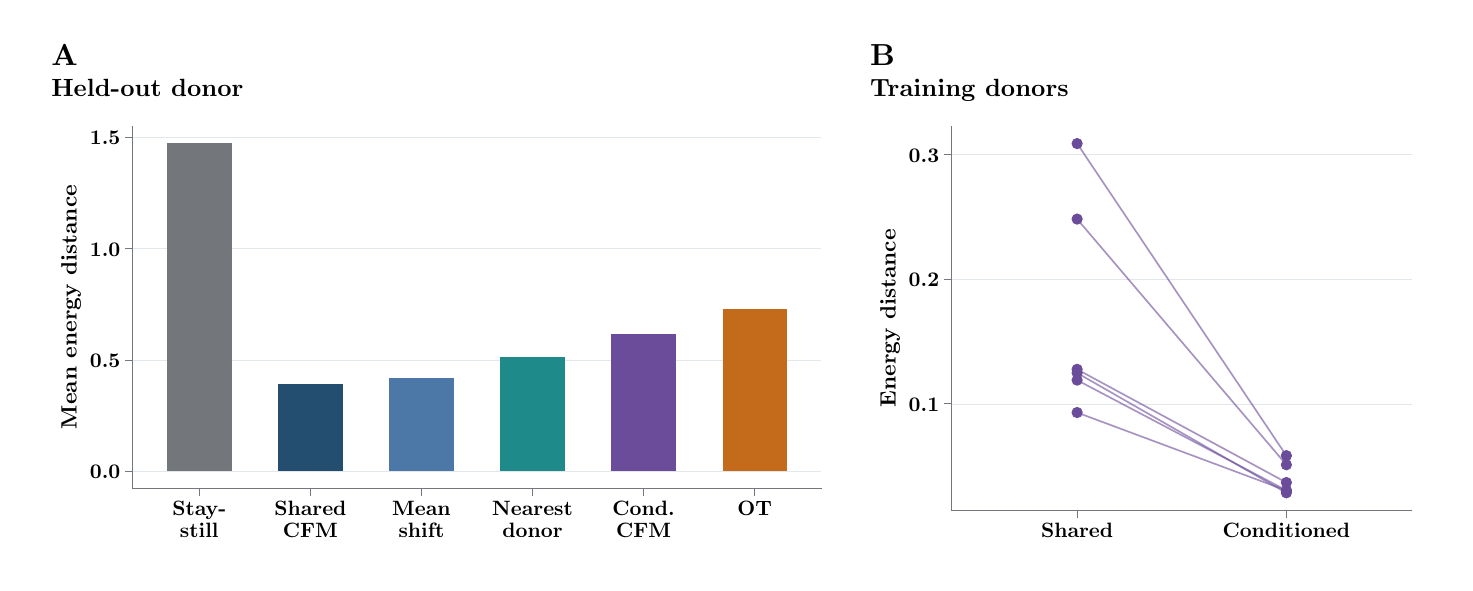
\begin{tikzpicture}[x=1pt,y=1pt]
\definecolor{fillColor}{RGB}{255,255,255}
\path[use as bounding box,fill=fillColor,fill opacity=0.00] (0,0) rectangle (512.15,193.48);
\begin{scope}
\path[clip] (  0.00,  0.00) rectangle (512.15,193.48);
\definecolor{drawColor}{RGB}{0,0,0}

\node[text=drawColor,anchor=base west,inner sep=0pt, outer sep=0pt, scale=  1.10] at (  8.54,179.91) {\bfseries A};

\node[text=drawColor,anchor=base west,inner sep=0pt, outer sep=0pt, scale=  0.90] at (  8.54,168.54) {\bfseries Held-out donor};
\end{scope}
\begin{scope}
\path[clip] (  8.54,  4.27) rectangle (290.22,163.03);
\definecolor{fillColor}{RGB}{255,255,255}

\path[fill=fillColor] (  8.54,  4.27) rectangle (290.22,163.03);
\end{scope}
\begin{scope}
\path[clip] ( 37.93, 27.17) rectangle (286.80,157.91);
\definecolor{fillColor}{RGB}{255,255,255}

\path[fill=fillColor] ( 37.93, 27.17) rectangle (286.80,157.91);
\definecolor{drawColor}{RGB}{226,231,235}

\path[draw=drawColor,line width= 0.2pt,line join=round] ( 37.93, 33.12) --
	(286.80, 33.12);

\path[draw=drawColor,line width= 0.2pt,line join=round] ( 37.93, 73.38) --
	(286.80, 73.38);

\path[draw=drawColor,line width= 0.2pt,line join=round] ( 37.93,113.64) --
	(286.80,113.64);

\path[draw=drawColor,line width= 0.2pt,line join=round] ( 37.93,153.90) --
	(286.80,153.90);
\definecolor{fillColor}{RGB}{115,119,123}

\path[fill=fillColor] ( 50.37, 33.12) rectangle ( 73.66,151.97);
\definecolor{fillColor}{RGB}{35,78,112}

\path[fill=fillColor] ( 90.51, 33.12) rectangle (113.80, 64.90);
\definecolor{fillColor}{RGB}{76,120,168}

\path[fill=fillColor] (130.66, 33.12) rectangle (153.94, 66.82);
\definecolor{fillColor}{RGB}{31,138,138}

\path[fill=fillColor] (170.80, 33.12) rectangle (194.08, 74.56);
\definecolor{fillColor}{RGB}{107,76,154}

\path[fill=fillColor] (210.94, 33.12) rectangle (234.22, 82.85);
\definecolor{fillColor}{RGB}{196,106,27}

\path[fill=fillColor] (251.08, 33.12) rectangle (274.36, 91.77);
\end{scope}
\begin{scope}
\path[clip] (  0.00,  0.00) rectangle (512.15,193.48);
\definecolor{drawColor}{RGB}{115,119,123}

\path[draw=drawColor,line width= 0.3pt,line join=round,line cap=rect] ( 37.93, 27.17) --
	( 37.93,157.91);
\end{scope}
\begin{scope}
\path[clip] (  0.00,  0.00) rectangle (512.15,193.48);
\definecolor{drawColor}{RGB}{0,0,0}

\node[text=drawColor,anchor=base east,inner sep=0pt, outer sep=0pt, scale=  0.75] at ( 33.49, 30.43) {\bfseries 0.0};

\node[text=drawColor,anchor=base east,inner sep=0pt, outer sep=0pt, scale=  0.75] at ( 33.49, 70.69) {\bfseries 0.5};

\node[text=drawColor,anchor=base east,inner sep=0pt, outer sep=0pt, scale=  0.75] at ( 33.49,110.96) {\bfseries 1.0};

\node[text=drawColor,anchor=base east,inner sep=0pt, outer sep=0pt, scale=  0.75] at ( 33.49,151.22) {\bfseries 1.5};
\end{scope}
\begin{scope}
\path[clip] (  0.00,  0.00) rectangle (512.15,193.48);
\definecolor{drawColor}{RGB}{115,119,123}

\path[draw=drawColor,line width= 0.3pt,line join=round] ( 35.09, 33.12) --
	( 37.93, 33.12);

\path[draw=drawColor,line width= 0.3pt,line join=round] ( 35.09, 73.38) --
	( 37.93, 73.38);

\path[draw=drawColor,line width= 0.3pt,line join=round] ( 35.09,113.64) --
	( 37.93,113.64);

\path[draw=drawColor,line width= 0.3pt,line join=round] ( 35.09,153.90) --
	( 37.93,153.90);
\end{scope}
\begin{scope}
\path[clip] (  0.00,  0.00) rectangle (512.15,193.48);
\definecolor{drawColor}{RGB}{115,119,123}

\path[draw=drawColor,line width= 0.3pt,line join=round,line cap=rect] ( 37.93, 27.17) --
	(286.80, 27.17);
\end{scope}
\begin{scope}
\path[clip] (  0.00,  0.00) rectangle (512.15,193.48);
\definecolor{drawColor}{RGB}{115,119,123}

\path[draw=drawColor,line width= 0.3pt,line join=round] ( 62.01, 24.33) --
	( 62.01, 27.17);

\path[draw=drawColor,line width= 0.3pt,line join=round] (102.16, 24.33) --
	(102.16, 27.17);

\path[draw=drawColor,line width= 0.3pt,line join=round] (142.30, 24.33) --
	(142.30, 27.17);

\path[draw=drawColor,line width= 0.3pt,line join=round] (182.44, 24.33) --
	(182.44, 27.17);

\path[draw=drawColor,line width= 0.3pt,line join=round] (222.58, 24.33) --
	(222.58, 27.17);

\path[draw=drawColor,line width= 0.3pt,line join=round] (262.72, 24.33) --
	(262.72, 27.17);
\end{scope}
\begin{scope}
\path[clip] (  0.00,  0.00) rectangle (512.15,193.48);
\definecolor{drawColor}{RGB}{0,0,0}

\node[text=drawColor,anchor=base,inner sep=0pt, outer sep=0pt, scale=  0.75] at ( 62.01, 17.36) {\bfseries Stay-};

\node[text=drawColor,anchor=base,inner sep=0pt, outer sep=0pt, scale=  0.75] at ( 62.01,  9.26) {\bfseries still};

\node[text=drawColor,anchor=base,inner sep=0pt, outer sep=0pt, scale=  0.75] at (102.16, 17.36) {\bfseries Shared};

\node[text=drawColor,anchor=base,inner sep=0pt, outer sep=0pt, scale=  0.75] at (102.16,  9.26) {\bfseries CFM};

\node[text=drawColor,anchor=base,inner sep=0pt, outer sep=0pt, scale=  0.75] at (142.30, 17.36) {\bfseries Mean};

\node[text=drawColor,anchor=base,inner sep=0pt, outer sep=0pt, scale=  0.75] at (142.30,  9.26) {\bfseries shift};

\node[text=drawColor,anchor=base,inner sep=0pt, outer sep=0pt, scale=  0.75] at (182.44, 17.36) {\bfseries Nearest};

\node[text=drawColor,anchor=base,inner sep=0pt, outer sep=0pt, scale=  0.75] at (182.44,  9.26) {\bfseries donor};

\node[text=drawColor,anchor=base,inner sep=0pt, outer sep=0pt, scale=  0.75] at (222.58, 17.36) {\bfseries Cond.};

\node[text=drawColor,anchor=base,inner sep=0pt, outer sep=0pt, scale=  0.75] at (222.58,  9.26) {\bfseries CFM};

\node[text=drawColor,anchor=base,inner sep=0pt, outer sep=0pt, scale=  0.75] at (262.72, 17.36) {\bfseries OT};
\end{scope}
\begin{scope}
\path[clip] (  0.00,  0.00) rectangle (512.15,193.48);
\definecolor{drawColor}{RGB}{0,0,0}

\node[text=drawColor,rotate= 90.00,anchor=base,inner sep=0pt, outer sep=0pt, scale=  0.80] at ( 17.68, 92.54) {\bfseries Mean energy distance};
\end{scope}
\begin{scope}
\path[clip] (  0.00,  0.00) rectangle (512.15,193.48);
\definecolor{drawColor}{RGB}{0,0,0}

\node[text=drawColor,anchor=base west,inner sep=0pt, outer sep=0pt, scale=  1.10] at (304.44,179.91) {\bfseries B};

\node[text=drawColor,anchor=base west,inner sep=0pt, outer sep=0pt, scale=  0.90] at (304.44,168.54) {\bfseries Training donors};
\end{scope}
\begin{scope}
\path[clip] (304.44,  4.27) rectangle (503.61,163.03);
\definecolor{fillColor}{RGB}{255,255,255}

\path[fill=fillColor] (304.44,  4.27) rectangle (503.61,163.03);
\end{scope}
\begin{scope}
\path[clip] (333.84, 19.07) rectangle (500.20,157.91);
\definecolor{fillColor}{RGB}{255,255,255}

\path[fill=fillColor] (333.84, 19.07) rectangle (500.20,157.91);
\definecolor{drawColor}{RGB}{226,231,235}

\path[draw=drawColor,line width= 0.2pt,line join=round] (333.84, 57.55) --
	(500.20, 57.55);

\path[draw=drawColor,line width= 0.2pt,line join=round] (333.84,102.58) --
	(500.20,102.58);

\path[draw=drawColor,line width= 0.2pt,line join=round] (333.84,147.61) --
	(500.20,147.61);
\definecolor{drawColor}{RGB}{107,76,154}

\path[draw=drawColor,draw opacity=0.60,line width= 0.6pt,line join=round] (379.21, 70.02) --
	(454.83, 29.12);

\path[draw=drawColor,draw opacity=0.60,line width= 0.6pt,line join=round] (379.21, 54.41) --
	(454.83, 26.24);

\path[draw=drawColor,draw opacity=0.60,line width= 0.6pt,line join=round] (379.21,124.32) --
	(454.83, 35.53);

\path[draw=drawColor,draw opacity=0.60,line width= 0.6pt,line join=round] (379.21, 68.72) --
	(454.83, 25.39);

\path[draw=drawColor,draw opacity=0.60,line width= 0.6pt,line join=round] (379.21,151.60) --
	(454.83, 38.83);

\path[draw=drawColor,draw opacity=0.60,line width= 0.6pt,line join=round] (379.21, 66.12) --
	(454.83, 26.28);
\definecolor{drawColor}{RGB}{107,76,154}
\definecolor{fillColor}{RGB}{107,76,154}

\path[draw=drawColor,line width= 0.3pt,line join=round,line cap=round,fill=fillColor] (379.21, 70.02) circle (  1.87);

\path[draw=drawColor,line width= 0.3pt,line join=round,line cap=round,fill=fillColor] (454.83, 29.12) circle (  1.87);

\path[draw=drawColor,line width= 0.3pt,line join=round,line cap=round,fill=fillColor] (379.21, 54.41) circle (  1.87);

\path[draw=drawColor,line width= 0.3pt,line join=round,line cap=round,fill=fillColor] (454.83, 26.24) circle (  1.87);

\path[draw=drawColor,line width= 0.3pt,line join=round,line cap=round,fill=fillColor] (379.21,124.32) circle (  1.87);

\path[draw=drawColor,line width= 0.3pt,line join=round,line cap=round,fill=fillColor] (454.83, 35.53) circle (  1.87);

\path[draw=drawColor,line width= 0.3pt,line join=round,line cap=round,fill=fillColor] (379.21, 68.72) circle (  1.87);

\path[draw=drawColor,line width= 0.3pt,line join=round,line cap=round,fill=fillColor] (454.83, 25.39) circle (  1.87);

\path[draw=drawColor,line width= 0.3pt,line join=round,line cap=round,fill=fillColor] (379.21,151.60) circle (  1.87);

\path[draw=drawColor,line width= 0.3pt,line join=round,line cap=round,fill=fillColor] (454.83, 38.83) circle (  1.87);

\path[draw=drawColor,line width= 0.3pt,line join=round,line cap=round,fill=fillColor] (379.21, 66.12) circle (  1.87);

\path[draw=drawColor,line width= 0.3pt,line join=round,line cap=round,fill=fillColor] (454.83, 26.28) circle (  1.87);
\end{scope}
\begin{scope}
\path[clip] (  0.00,  0.00) rectangle (512.15,193.48);
\definecolor{drawColor}{RGB}{115,119,123}

\path[draw=drawColor,line width= 0.3pt,line join=round,line cap=rect] (333.84, 19.07) --
	(333.84,157.91);
\end{scope}
\begin{scope}
\path[clip] (  0.00,  0.00) rectangle (512.15,193.48);
\definecolor{drawColor}{RGB}{0,0,0}

\node[text=drawColor,anchor=base east,inner sep=0pt, outer sep=0pt, scale=  0.75] at (329.39, 54.86) {\bfseries 0.1};

\node[text=drawColor,anchor=base east,inner sep=0pt, outer sep=0pt, scale=  0.75] at (329.39, 99.89) {\bfseries 0.2};

\node[text=drawColor,anchor=base east,inner sep=0pt, outer sep=0pt, scale=  0.75] at (329.39,144.93) {\bfseries 0.3};
\end{scope}
\begin{scope}
\path[clip] (  0.00,  0.00) rectangle (512.15,193.48);
\definecolor{drawColor}{RGB}{115,119,123}

\path[draw=drawColor,line width= 0.3pt,line join=round] (330.99, 57.55) --
	(333.84, 57.55);

\path[draw=drawColor,line width= 0.3pt,line join=round] (330.99,102.58) --
	(333.84,102.58);

\path[draw=drawColor,line width= 0.3pt,line join=round] (330.99,147.61) --
	(333.84,147.61);
\end{scope}
\begin{scope}
\path[clip] (  0.00,  0.00) rectangle (512.15,193.48);
\definecolor{drawColor}{RGB}{115,119,123}

\path[draw=drawColor,line width= 0.3pt,line join=round,line cap=rect] (333.84, 19.07) --
	(500.20, 19.07);
\end{scope}
\begin{scope}
\path[clip] (  0.00,  0.00) rectangle (512.15,193.48);
\definecolor{drawColor}{RGB}{115,119,123}

\path[draw=drawColor,line width= 0.3pt,line join=round] (379.21, 16.23) --
	(379.21, 19.07);

\path[draw=drawColor,line width= 0.3pt,line join=round] (454.83, 16.23) --
	(454.83, 19.07);
\end{scope}
\begin{scope}
\path[clip] (  0.00,  0.00) rectangle (512.15,193.48);
\definecolor{drawColor}{RGB}{0,0,0}

\node[text=drawColor,anchor=base,inner sep=0pt, outer sep=0pt, scale=  0.75] at (379.21,  9.26) {\bfseries Shared};

\node[text=drawColor,anchor=base,inner sep=0pt, outer sep=0pt, scale=  0.75] at (454.83,  9.26) {\bfseries Conditioned};
\end{scope}
\begin{scope}
\path[clip] (  0.00,  0.00) rectangle (512.15,193.48);
\definecolor{drawColor}{RGB}{0,0,0}

\node[text=drawColor,rotate= 90.00,anchor=base,inner sep=0pt, outer sep=0pt, scale=  0.80] at (313.59, 88.49) {\bfseries Energy distance};
\end{scope}
\end{tikzpicture}

\end{document}
